\documentclass[a4paper,14pt]{extreport}
\usepackage[left=30mm,right=10mm,top=20mm,bottom=20mm]{geometry}
\parindent 1.25cm
\linespread{1.5}

\usepackage{cmap}
\usepackage{lipsum}
\usepackage{chngcntr}\counterwithout{table}{chapter}

\usepackage[utf8]{inputenc}
\usepackage[T2A]{fontenc}
\usepackage[english,russian]{babel}
\usepackage{fontspec}
\setmainfont{Times New Roman}

\usepackage{indentfirst}

\usepackage[backend=biber,style=gost-numeric]{biblatex}
\addbibresource{biblio.bib}

\usepackage{multicol}
\usepackage{listings}
\usepackage{graphicx}
\graphicspath{ {assets/} }
\usepackage{placeins}
\usepackage{multirow}
\usepackage{paralist}
\usepackage{float}

\usepackage{longtable}
\usepackage{makecell}
\usepackage{pgfplots}
\usepackage{pgfplotstable}
\usepackage{caption, subcaption}
\captionsetup[table]{justification=raggedright,singlelinecheck=false}

\usepackage{xltabular, tabularx}

\usepackage{fancyhdr}
\pagestyle{fancy}
\renewcommand{\headrulewidth}{0pt}
\fancyhf{}
\fancyfoot[C]{\thepage}

\fancypagestyle{plain} {
	\renewcommand{\headrulewidth}{0pt}
	\fancyhf{}
  \fancyfoot[C]{\thepage}
}

\usepackage{titletoc, amsmath, lastpage} %подключаем нужные пакеты расширений
\usepackage{amsfonts} % для mathbb и пр.
\usepackage[raggedright]{titlesec} % не переносить заголовки

\titleformat{\chapter}[block]{\centering\Large\bfseries}{\MakeUppercase{\chaptertitlename}\ \thechapter . }{0pt}{\MakeUppercase}
\titlespacing{\chapter}{0pt}{10pt}{6pt}

\titleformat{\section}[block]{\centering\Large\bfseries}{\thesection . }{0pt}{}
\titlespacing{\section}{0pt}{10pt}{3pt}

\titleformat{\subsection}[block]{\centering\Large\bfseries\itshape}{\thesubsection . }{0pt}{}

\titleformat{\subsubsection}[block]{\centering\itshape}{\thesubsubsection . }{0pt}{}

\titleformat{\paragraph}[block]{\bfseries}{\theparagraph .}{0pt}{}
\titlespacing{\paragraph}{0pt}{10pt}{0pt}


% TABLE OF CONTENT CONFIG
\usepackage{tocloft}

% disables bold in table of content
\newcommand*{\disableboldchapterintoc}{%
	\addtocontents{toc}{\string\renewcommand{\protect\cftchappagefont}{\protect\normalfont}}
	\addtocontents{toc}{\string\renewcommand{\protect\cftchapfont}{\protect\normalfont}}
	\addtocontents{toc}{\string\renewcommand{\protect\cftchapleader}{\protect\normalfont\protect\cftdotfill{\protect\cftsecdotsep}}}%
}

\renewcommand{\cftaftertoctitle}{\hfill}

\setlength{\cftchapindent}{0pt}
\setlength{\cftsecindent}{0pt}
\setlength{\cftsubsecindent}{0pt}
\cftsetindents{section}{0pt}{1.0\baselineskip}
\cftsetindents{chapter}{0pt}{1.0\baselineskip}

\titlecontents{chapter}[0pt]{}{\chaptername\ \thecontentslabel. }{}{\cftdotfill{\cftsecdotsep}\contentspage}

\titlelabel{\thetitle.\quad}

\renewcommand{\cftdotsep}{1}

\makeatletter
\renewcommand\chapter{\par%
  \thispagestyle{plain}%
  \global\@topnum\z@
  \@afterindentfalse
  \secdef\@chapter\@schapter}
\makeatother

\makeatletter
\renewcommand\large{\@setfontsize\large{14}{16}}
\renewcommand\Large{\@setfontsize\Large{14}{16}}
\renewcommand\Large{\@setfontsize\LARGE{14}{16}}
\makeatother

\usepackage{xargs}
\newcommandx{\fig}[4][1=, 2=1, 3=]{
  \begin{figure}[H]
    \centering
    \includegraphics[width=#2\textwidth]{#4}
    \caption{#1}
    \label{#3}
  \end{figure}
}

\newcommand{\refAppendix}[1]{
  (Приложение \ref{#1})
}

\newcommand{\refImg}[1]{
  (рис. \ref{#1})
}

\usepackage{placeins} % floatbarrier
\usepackage{setspace} %line spacing

\usepackage{enumitem}
\setlist[itemize]{noitemsep, topsep=0pt}
\setlist[enumerate]{noitemsep, topsep=0pt}

% Меняем везде перечисления на цифра.цифра
\renewcommand{\theenumi}{\arabic{enumi}.}
\renewcommand{\labelenumi}{\arabic{enumi}.}
\renewcommand{\theenumii}{.\arabic{enumii}.}
\renewcommand{\labelenumii}{\hspace*{1cm}\arabic{enumi}.\arabic{enumii}.}
\renewcommand{\theenumiii}{.\arabic{enumiii}.}
\renewcommand{\labelenumiii}{\arabic{enumi}.\arabic{enumii}.\arabic{enumiii}.}

\renewcommand{\cellalign}{vh}
\renewcommand{\theadalign}{vh}

\newcommand{\chaperWONum}[1]{\chapter*{#1}\addcontentsline{toc}{chapter}{#1}}
\renewcommand\thesubfigure{\asbuk{subfigure}}

\lstset{ %
language=java,                % выбор языка для подсветки (здесь это С)
basicstyle=\small\sffamily,   % размер и начертание шрифта для подсветки кода
numbers=left,                 % где поставить нумерацию строк (слева\справа)
numberstyle=\tiny,            % размер шрифта для номеров строк
stepnumber=1,                 % размер шага между двумя номерами строк
firstnumber=1,
numberfirstline=true
numbersep=5pt,                % как далеко отстоят номера строк от подсвечиваемого кода
backgroundcolor=\color{white},% цвет фона подсветки - используем \usepackage{color}
showspaces=false,             % показывать или нет пробелы специальными отступами
showstringspaces=false,       % показывать или нет пробелы в строках
showtabs=false,               % показывать или нет табуляцию в строках
frame=single,                 % рисовать рамку вокруг кода
tabsize=2,                    % размер табуляции по умолчанию равен 2 пробелам
captionpos=t,                 % позиция заголовка вверху [t] или внизу [b]
breaklines=true,              % автоматически переносить строки (да\нет)
breakatwhitespace=false,      % переносить строки только если есть пробел
escapeinside={\%*}{*)}        % если нужно добавить комментарии в коде
}

% сюда можно помещать свои настройки не редактируя main, чтоб не решать проблему с мёрджем при изменение шаблона


\begin{document}
  \selectlanguage{russian}

  \newcommand{\Author}{Поздняков А. А.} % ФИО автора
\newcommand{\AuthorFull}{Поздняков Артемий Анатольевич} % ФИО автора
\newcommand{\Supervisor}{Фёдоров С. А.} % ФИО руководителя
\newcommand{\SupervisorFull}{Фёдоров Станислав Алексеевич}
\newcommand{\SupervisorPosition}{старший преподаватель ВШПИ ИКНК}
\newcommand{\ProfileCode}{09.03.04}
\newcommand{\ProfileName}{Программная инженерия}
\newcommand{\ConsultantNorm}{Локшина Е. Г.} %ФИО нормконтроль
\newcommand{\TaskCreatedBukvami}{''18'' апреля 2024 г.}
\newcommand{\TaskCreatedCiframi}{18.04.2024}
\newcommand{\TaskDeadline}{20.05.2024}

\newcommand{\Theme}{Сравнение методов сжатия атрибутов облаков точек} %тема диплома
\newcommand{\Group}{5130904/00104} %группа

  \pagenumbering{gobble}

  \begin{spacing}{1}
    \begin{titlepage}

  \begin{center} % Center everything on the page

    %----------------------------------------------------------------------------------------
    %	HEADING SECTIONS
    %----------------------------------------------------------------------------------------



    Министерство образования и науки Российской Федерации\\
    Санкт-Петербургский политехнический университет Петра Великого\\
    Институт компьютерных наук и технологий\\
    Высшая школа программной инженерии\\[0.9cm]


    \begin{minipage}{\linewidth}
      \begin{tabularx}{\linewidth}{X@{}l@{}}
         & Работа допущена к защите                                                               \\
         & Директор ВШПИ                                                                          \\
         & \underline{\hspace*{0.1\textheight}} П. Д. Дробинцев                                   \\
         & <<\underline{\hspace*{0.05\textheight}}>> \underline{\hspace*{0.1\textheight}} 2022~г. \\
      \end{tabularx}
    \end{minipage}\\[1.5cm]

    {\Large \bfseries ВЫПУСКНАЯ КВАЛИФИКАЦИОННАЯ РАБОТА}\\
    {\Large \bfseries работа бакалавра}\\[1.5cm]

    %----------------------------------------------------------------------------------------
    %	TITLE SECTION
    %----------------------------------------------------------------------------------------

    {\Large \bfseries \MakeUppercase{\Theme}}\\[0.4cm] % Title of your document

    {
    \begin{flushleft}
      по направлению подготовки (специальности)\\
      09.03.04 Программная инженерия\\[0.2cm]
      Направленность (профиль)\\
      09.03.04\_1 «Технология разработки и сопровождения качественного программного продукта»\\[0.6cm]
    \end{flushleft}
    }

    \bigskip
    %----------------------------------------------------------------------------------------
    %	AUTHOR SECTION
    %----------------------------------------------------------------------------------------
    {
      \begin{tabularx}{\linewidth}{@{}>{\raggedright}p{5cm} X @{}r@{}}
        Выполнил студент гр. \Group        & \hspace{10cm} & \Author         \\[2\baselineskip]
        Руководитель старший преподаватель & \hspace{10cm} & \Supervisor     \\[2\baselineskip]
        Консультант по нормоконтролю       & \hspace{10cm} & \ConsultantNorm \\
      \end{tabularx}
    }

    \vfill


    \centering{
      Санкт-Петербург\\
      2022
    }
  \end{center}
\end{titlepage}
\newpage
% \cleardoublepage

  \end{spacing}


  \newpage
  \begin{center}
  {САНКТ-ПЕТЕРБУРГСКИЙ ПОЛИТЕХНИЧЕСКИЙ УНИВЕРСИТЕТ\\ ПЕТРА ВЕЛИКОГО} \\
  {Институт компьютерных наук и технологий} \\
  {Высшая школа программной инженерии} \\

  {
  \begin{flushright}
    УТВЕРЖДАЮ\\
    Директор ВШПИ\\
    \underline{\hspace{2.2cm}} П.Д. Дробинцев\\
    \TaskCreatedBukvami\\[1.8cm]
  \end{flushright}
  }

  \textbf{ЗАДАНИЕ} \\
  \textbf{на выполнение выпускной квалификационной работы}\\
  студенту \AuthorFull, группа \Group \\[0.5cm]
  \begin{enumerate}[label=\arabic*.]
    \item Тема работы: \Theme
    \item Срок сдачи студентом законченной работы: \TaskDeadline
    \item Исходные данные по работе:
      \begin{itemize}
        \item Документация на язык программирования Python;
        \item Документация к библиотеке Open3D;
        \item Документация к библиотеке NumPy;
      \end{itemize}
    \item Содержание работы (перечень подлежащих разработке вопросов):
      \begin{itemize}
        \item Обоснование актуальности работы
        \item Обзор существующих решений
        \item Составление требований к разрабатываемому решению
        \item Описание реализации
        \item Анализ результатов
      \end{itemize}
    \item Перечень графического материала (с указанием обязательных чертежей):
    \item Консультанты по работе:
    \item Дата выдачи задания: \TaskCreatedCiframi
  \end{enumerate}
\end{center}
Руководитель ВКР \hspace{3.5cm} \underline{\hspace{5cm}} \hfill \Supervisor\\[0.5cm]
Задание принял к исполнению \TaskCreatedCiframi\\[0.5cm]
Студент \hspace{5.8cm} \underline{\hspace{5cm}} \hfill \Author\\


  \newpage
  \sloppy

  \chapter*{Реферат}
    На 52 с., 10 рисунков, 4 таблицы.

КЛЮЧЕВЫЕ СЛОВА: PCC, POINT CLOUD COMPRESSION, ОБЛАКО ТОЧЕК, СЖАТИЕ, БЕНЧМАРК

Тема выпускной квалификационной работы: ''Сравнение методов сжатия атрибутов
облаков точек''.

Бакалаврская работа посвящена разработке подхода к оценке различных методов
сжатия атрибутов облаков точек. Дан обзор существующих систем оценки качества
сжатия облаков точек. Определён набор метрик для сравнения методов сжатия
облаков точек и их атрибутов. В результате анализа существующих решений,
определён набор требований для новой системы оценки методов сжатия атрибутов
облаков точек.

В рамках работы была разработана программа для вычисления качественных метрик
сжатия облаков точек с использования языка Python. Предложенное решение было
внедрёно в существующую систему бенчмаркинга кодеков для сжатия облаков точек
PCCArena. С помощью модифицированной системы PCCArena произведён качественный
сравнительный анализ кодеков Draco и TMC13.


    \newpage
  \chapter*{Abstract}
    \begin{otherlanguage}{english}
      52 pages, 10 figures, 4 tables.

KEYWORDS: PCC, POINT CLOUD COMPRESSION, POINT CLOUD, COMPRESSION, BENCHMARK

The topic of final qualifying work: ''Comparison of point cloud attribute
compression methods''.

This Bachelor's work describes the development of the new approach for
comparison of different point cloud attribute compression methods. In this
paper, the analysis of existing point cloud compression quality assessment
systems carried out. Also, the suite of metrics for point cloud attribute
compression is defined. As a result of existing approaches analysis, the suite
of requirements for new point cloud compression quality assessment system is
defined.

In the course of work, the software for evaluating point cloud compression
qualitative metrics was developed using Python programming language. The
proposed approach was integrated into PCCArena - point cloud compression
benchmark. Using modified version of PCCArena, qualitative comparative analysis
of Draco and TMC13 codecs carried out.
    \end{otherlanguage}

    \newpage
    \disableboldchapterintoc
    \renewcommand{\contentsname}{\textbf{СОДЕРЖАНИЕ}}
    \renewcommand{\cfttoctitlefont}{\hfill\Large}

    \tableofcontents
    \newpage

    \pagenumbering{arabic}
    \setcounter{page}{6}

    % введение
    \chaperWONum{Введение}
    \textbf{Облака точек}. Растущая популярность (?ссылка?) технологий компьютерного
зрения (CV - Computer Vision) и расширенной реальности (XR - eXtended Reality)
влечёт за собой потребность в способах компактного хранения и передачи
трёхмерных (далее 3Д) данных. 3Д-данные представляются в виде полигональных
сеток - совокупности вершин, рёбер и граней, определяющих форму трёхмерного
объекта, или облаков точек, отличающихся от последних отсутствием связей между
вершинами. Дополнительно, данные о геометрической структуре объекта могут быть
дополнены информацией о его внешних характеристиках.

Важной задачей является создание цифрового представления реальных объектов и
сцен. 3Д-сканирование - технология, позволяющая считывать форму физического
объекта и его внешних характеристик, таких как цвет или отражающая способность
поверхности. В общем случае, результатом процесса 3Д-сканирования является
конечное множество точек в трёхмерном
пространстве\cite[10]{SurfaceReconstruction}.

Полигональные сетки аппроксимируют непрерывную поверхность исходного объекта. В
свою очередь, облака точек сохраняют мельчайшие подробности структуры
поверхности объекта вплоть до миллиметра\cite[33]{SurfaceReconstruction}. Задача
получения 3Д-модели объекта в виде полигональной сетки по имеющемуся облаку
точек, считанных с его поверхности, решается методами реконструкции
поверхности\cite{SurfaceReconstruction}. Для обратного преобразования достаточно
удалить связи между вершинами в полигональной сетке.

Большая точность позволяет использовать облака точек для машинной обработки в
системах компьютерного зрения, взаимодействующих с реальным миром. Примером
подобных систем являются беспилотные автомобили, использующие лидары - локаторы,
испускающие световые волны оптического диапазона с дальнейшей регистрацией
отраженных импульсов\cite[7]{PointCloudAnalysis}. Другим примером являются
системы расширенной реальности, в данном случае облака точек используются для
совмещения позиций виртуальных объектов и физических объектов, находящихся рядом
с человеком\cite[15]{PointCloudAnalysis}.

Для точного описания поверхности, облака точек должны быть достаточно плотными.
Точки в облаке представляют собой дискретные образцы непрерывной поверхности, а
полигональные сетки аппроксимируют данную поверхность
полигонами\cite[4]{PointCloudAnalysis}. Всё это влечёт за собой большой размер
облаков точек (может тут тоже ссылка?), в связи с чем возникает задача
разработки способов компактного хранения подобных объектов.

Алгоритмы сжатия облаков точек решают задачу компактного хранения и передачи
облаков точек. Популярные кодеки были реализованы в рамках проектов
Draco\cite{Draco} и PCL\cite{Rusu_ICRA2011_PCL}. В настоящее время различными
авторами предлагаются новые методы сжатия геометрической структуры облаков
точек\cite{PCGCv2}\cite{GeoCNNv2} и их
атрибутов\cite{Shao2017}\cite{Chen2020}\cite{Sun2023}. Алгоритм кодирования
данных в этих решениях можно разделить на этапы реконструкции изначальной
геометрической структуры объекта и кодирования атрибутов облака в соответствии с
полученной структурой. Работа по стандартизации PCC-кодеков была начата MPEG в
2017 году\cite{CallForProposalV2}, также данной группой был предложен
собственный кодек и разработана тестовая модель на его основе -
TMC13\cite{TMC13}.

Большое количество постоянно появляющихся подходов к сжатию облаков точек делает
актуальной задачу разработки программы для оценки работы PCC-кодеков. Подобная
программа может быть использована исследователями для подсчёта метрик
разрабатываемых ими кодеков.

\textbf{Цель работы} - разработка подхода к сравнению алгоритмов сжатия
атрибутов облаков точек. В рамках данной работы необходимо решить следующие
задачи:

\begin{itemize}
    \item Проанализировать системы оценки качества сжатия облаков точек
    \item Изучить релевантные метрики, отображающие эффективность и качество
    сжатия атрибутов облаков точек
    \item Разработать программу подсчёта метрик
    \item Получить метрики для отобранных PCC-кодеков
    \item Проанализировать результаты работы
\end{itemize}

% \textbf{Алгоритмы сжатия облаков точек}.  Алгоритмы сжатия облаков точек
% (PCC-алгоритмы - Point Cloud Compression алгоритмы) можно классифицировать по
% следующим признакам:

% \begin{itemize}
%     \item Signal Processing / ML-based\cite{Wu2020}
%     \item С потерями / без потерь геометрии\cite{CallForProposalV2}
%     \item С потерями / без потерь атрибутов\cite{CallForProposalV2}
% \end{itemize}


    \newpage
\chapter{Обзор подходов к сравнению методов сжатия облаков точек}

% что такое лузлес
% что такое лосси

В общем случае, информация может быть сжата, если она является избыточной.
Сжатие без потерь основано на уменьшения избыточности информации. В сжатии с
потерями вводится новое понятие - нерелевантная информация, то есть такая
информация, которая слабо влияет на восприятие изображения человеком. Сжатие с
потерями, таким образом, основано не только на уменьшении избыточности, но и на
определении нерелевантной информации и уменьшении количества подобной
информации\cite[265]{DataCompression}.

В случае, когда визуальная информация предназначена прежде всего для восприятия
человеком, единственной корректной метрикой визуального качества изображения
является субъективная оценка некоторой отобранной группой
людей\cite{SSIMArticle}. Данный подход, однако, не является машинным и,
следовательно, не подлежит автоматизации. Для решения данной проблемы были
разработаны метрики, помогающие автоматически предсказать \textit{воспринимаемое
качество (perceived quality)} изображения. К подобным метрикам относится метрики
качества изображения SSIM и VIF.

\section{Подходы к оценке качества сжатия изображений}

% мб сабсекции?
% перцепчуал метрики
% не перцепчуал метрики

Потребность в оценке качества сжатия визуальной информации возникла после
изобретения методов сжатия подобной информации. Многие из качественных метрик
сжатия 3Д-данных, были изначально разработаны для оценки качества сжатия обычных
изображений.

Введем понятие реконструированного изображения. Пусть оригинальное изображение
$A$ было закодировано в формате $F_{1}$. Закодируем оригинальное изображение с
использованием алгоритма сжатия и получим сжатое изображение $B$, закодированное
в формате $F_{2}$. Теперь произведем декомпрессию изображения $B$ и закодируем
его с помощью формата $F_{1}$. Полученное изображение $C$ в формате $F_{1}$ -
реконструированное изображение.

Метрики качества для медиа могут быть классифицированы по признаку доступности
исходного изображения\cite{SSIMArticle}:

\begin{itemize}
    \item Оригинальное неискаженное изображение доступно
    \item Доступен лишь набор признаков, извлеченных из оригинального изображения
    \item Оригинальное изображение недоступно
\end{itemize}

Другая классификация предполагает разделение метрик по признаку того, на чём они
основаны\cite[6]{FullReferenceIQMetrics}:

\begin{itemize}
    \item Математически-обоснованные метрики, учитывающие лишь интенсивность
    искажения. К подобным метрикам относятся среднеквадратичная ошибка (MSE) и
    отношение пикового сигнала к шуму (PSNR)
    \item Низкоуровневые метрики, которые учитывают видимость искажений, как,
    например функции чувствительности контраста (CSF)
    \item Высокоуровневые метрики, которые основаны на гипотезе о том, что
    человеческое зрение адаптировано к извлечению структурной информации из
    изображения. К подобным метрикам относится индекс структурной похожести
    (SSIM) и визуальная точность изображения (VIF)
\end{itemize}

\subsection{Математически-обоснованные метрики качества}

Одной из стандартных метрик качества сжатия изображений является отношение
пикового сигнала к шуму (Peak Signal to Noise Ratio - далее PSNR). Данная
метрика достаточно проста для вычисления, однако она имеет лишь ограниченное,
приблизительное отношение к ошибкам, которые воспринимает человеческий глаз.
Иными словами, большее значение PSNR означает меньшее расхождение между
оригинальным и сжатым изображением, но не гарантирует положительное восприятие
реконструированного изображения человеком\cite[279]{DataCompression}.

Обозначим пиксели исходного изображения как $P_{i}$, а пиксели
реконструированного изображения как $Q_{i}$ $\left(\text{где} \ 0 \le i \le
n\right)$. Для начала определим понятие среднеквадратичной ошибки (Mean Squared
Error - далее MSE) между двумя изображениями как

\begin{equation} \label{eq:img_mse}
    MSE = \frac{1}{n} \sum_{i=1}^{n}\left(P_{i} - Q_{i}\right)^2
\end{equation}

Иными словами, среднеквадратичная ошибка для изображений является суммой
квадратов ошибок для каждого из пикселей, разделённой на общее количество точек.
Тогда метрика PSNR может быть определена как

\begin{equation} \label{eq:img_psnr}
    \text{PSNR} = 10\log_{10} \frac{\max_{i}\left|P_{i}\right|^{2}}{MSE}
\end{equation}

При этом $\max_{i}\left|P_{i}\right|$ - пиковое значение сигнала. Для
чёрно-белого изображения пиковым значением является 1, для изображения в
оттенках серого при глубине 8 бит на пиксель данное значение равно 255. Так как
используется логарифм отношения, итоговое значение измеряется в децибелах.

% Метрика PSNR имеет значение лишь в сравнении c показателями данной метрики для
% того же (или схожего) кодека и тех же входных данных при отличных входных
% параметрах\cite{HuynhThu2008}. Несмотря на это, данная метрика продолжает
% использоваться исследователями для сравнения качества работы существующих
% кодеков с предлагаемыми ими решениями\cite{NetflixVMAFMedium}.

Другой похожей метрикой является отношение сигнала к шуму (Signal to Noise Ratio
- далее SNR). В данном случае, рассматривается не пиковое значение сигнала, а
среднеквадратичное.

\begin{equation} \label{eq:img_snr}
    \text{SNR} = 10\log_{10} \frac{\frac{1}{n}\sum_{i=1}^{n} P_{i}^{2}}{MSE}
\end{equation}

Значение отношения сигнала к шуму квантования (Signal to Quantization Noise
Ratio - далее SQNR) представляет собой меру влияния квантования на качество
сигнала. Данную метрику можно определить как отношение мощности сигнала к
разнице между сигналом после квантования и оригинальным значением сигнала.

\begin{equation} \label{eq:img_sqnr}
    \text{SQNR} = 10\log_{10} \frac{\text{signal power}}{\text{quantization error}}
\end{equation}

\subsection{Высокоуровневые метрики качества}

% мощности шума?

Математически-обоснованные метрики основаны на предположении, что уменьшение
воспринимаемого качества изображения напрямую связано с величиной шума. Так,
например, MSE даёт объективную оценку мощности шума, однако два зашумленных
изображения с одинаковым значением MSE могут иметь ошибки разного рода,
некоторые из которых являются более заметными чем другие. Для решения данной
проблемы были предложены высокоуровневые метрики качества изображений.

% Здесь можно стырить иллюстрацию с лодками из\cite{SSIMArticle}.

% ниже chatgpt

Рассмотрим индекс структурной похожести (SSIM), данная метрика была предложена в
качестве способа предсказания воспринимаемого качества изображения. Она
представляет собой более точную и соответствующую человеческому восприятию
метрику для оценки качества сжатия изображений, поскольку учитывает структурные
и текстурные аспекты изображения, в то время как MSE и PSNR ориентированы на
разницу в значениях пикселей без учета визуальных особенностей.

% ниже chatgpt

\subsection{SSIM (Structural Similarity Index)}

Вычисляется сравнением трех основных аспектов изображений: яркости (luminance),
контрастности (contrast) и структуры (structure). Вот формула для вычисления
SSIM:

\begin{equation} \label{eq:img_ssim}
    \text{SSIM}\left(x, y\right) = \frac{
        \left(2\mu_{x}\mu_{y} + c_{1}\right)\left(2\sigma_{xy} + c_{2}\right)
    }{
        \left(\mu_{x}^{2} + \mu_{y}^2 + c_{1}\right)\left(\sigma_{x}^{2} + \sigma_{y}^{2} + c_{2}\right)
    }
\end{equation}

\noindent где:

\begin{itemize}
    \item $x$ и $y$ - сравниваемые изображения
    \item $\mu_{x}$ и $\mu_{y}$​ - средние значения пикселей изображений $x$ и $y$
    \item $\sigma_{x}^{2}$ и $\sigma_{y}^{2}$ - дисперсии значений пикселей изображений $x$ и $y$
    \item $\sigma_{xy}$ - ковариация между значениями пикселей изображений $x$ и $y$
    \item $c_{1}$ и $c_{2}$ - константы для обеспечения устойчивости деления
\end{itemize}

% ниже chatgpt

Этот индекс обычно принимает значения от $-1$ до $1$, где $1$ указывает на
идеальное сходство между изображениями, а значения ближе к $-1$ указывают на
более сильные различия.

% ниже chatgpt

SSIM сравнивает локальные окрестности пикселей изображений, а не их абсолютные
значения. Он учитывает не только яркость и контрастность, но и структуру
изображения, что делает его более подходящим для оценки качества изображений с
точки зрения человеческого восприятия

% ниже chatgpt

\subsection{VIF (Visual Information Fidelity)}

VIF обеспечивает более точную оценку качества сжатия, так как учитывает не
только структурные аспекты изображения, но и сложные визуальные особенности,
такие как текстуры, края и детали. Это делает VIF более подходящей метрикой для
оценки реального восприятия качества изображения человеком.

% ниже chatgpt

Вычисление Visual Information Fidelity (VIF) включает несколько этапов,
включающих оценку сходства между двумя изображениями с учетом их визуальной
информации. Вот общий алгоритм вычисления VIF:

\begin{itemize}
    \item Разбиение изображений на блоки: Сначала изображения разбиваются на
    небольшие блоки пикселей. Обычно используются квадратные блоки определенного
    размера.
    \item Вычисление локальных статистических параметров: Для каждого блока
    изображения вычисляются локальные статистические параметры, такие как
    среднее значение, дисперсия и ковариация пикселей.
    \item Вычисление локальных масштабных параметров: Для каждого блока
    изображения также вычисляются локальные масштабные параметры, которые
    оценивают структурную информацию в блоке.
    \item Вычисление глобальных статистических параметров: Глобальные
    статистические параметры вычисляются на основе суммирования или усреднения
    локальных параметров по всем блокам изображений.
    \item Вычисление VIF: Затем производится расчет VIF, используя локальные
    и глобальные параметры. В общем, VIF представляет собой взвешенную сумму
    сходства между локальными статистическими параметрами двух изображений.
    \item Нормализация VIF: Иногда VIF может быть нормализован для получения
    значения в диапазоне от 0 до 1, где 1 указывает на идеальное сходство между
    изображениями.
\end{itemize}

% ниже chatgpt

Это общий алгоритм, и реальная реализация VIF может включать дополнительные
детали и оптимизации. Однако основная идея заключается в том, чтобы учитывать
как локальные, так и глобальные статистические параметры изображений для оценки
их визуального сходства.

% ниже chatgpt

В целом, VIF обеспечивает более глубокую и точную оценку качества сжатия
изображений, учитывая разнообразные визуальные особенности и взаимосвязи между
блоками изображения, что делает его ценным инструментом при сравнении различных
методов сжатия изображений.

% \subsection{Netflix VMAF}

\section{Подходы к оценке качества сжатия облаков точек}

% Ввести в область и рассказать про метрики фото, видео

% Классифицировать метрики

% Рассказать как их адаптировать для пойнт клаудов

Идея многих подходов к оценке качества сжатия облаков точек взята из более
глубоко проработанной области оценки качества изображений и видео. Облака точек,
однако представляют собой гораздо более сложный объект, что влияет не только на
то, какие стандартные математически-обоснованные качественные метрики можно к
ним применить, но и на сам процесс вычисления данных метрик. Рассмотрим
терминологию, связанную с наличием потерь при сжатии облаков
точек\cite{CallForProposalV2}:

\begin{itemize}
    \item Преобразование геометрической структуры с потерями. Координаты точек в
    декодированном облаке не обязательно численно совпадают с изначальными
    координатами. Количество точек в декодированном облаке также может не
    совпадать с количеством точек в изначальном облаке
    \item Преобразование геометрической структуры без потерь. Координаты точек в
    декодированном облаке численно совпадают с изначальными координатами.
    Количество точек в декодированном облаке также совпадает с количеством точек
    в изначальном облаке
    \item Преобразование атрибутов с потерями. Декодированные сжатые атрибуты не
    обязательно численно совпадают с изначальными атрибутами
    \item Преобразование атрибутов без потерь. Декодированные сжатые атрибуты
    полностью численно совпадают с изначальными атрибутами
\end{itemize}

Очевидно, что метрики качества релевантны только для методов сжатия
геометрической структуры с потерями и методов сжатия атрибутов с потерями.
Рассмотрим, как некоторые из вышеупомянутых метрик можно адаптировать для оценки
качества сжатия облаков точек.

% мб вот эту матемагию для 2-3 части оставить?
% а здесь описать то же самое словами

Искажение геометрической структуры можно оценить, вычислив среднеквадратичную
ошибку искажения. Для этого необходимо определить, что собой представляет ошибка
для единичной точки. Точку оригинального облака назовём оригинальной точкой,
данная точка в ходе сжатия с потерями и последующей декомпрессии определенным
образом преобразуется, соответствующую точку в реконструированном облаке назовём
реконструированной точкой. Возможно несколько случаев:

\begin{enumerate}
    \item Координаты оригинальной и реконструированной точки полностью совпадают
    \item Координаты оригинальной и реконструированной точки отличаются
    незначительно
    \item Реконструированной точки не существует. Сжатия с потерями
    геометрической структуры не гарантирует совпадение количества точек в
    оригинальном и реконструированном облаке, соответственно, исходная точка
    может быть редуцирована или заменена несколькими другими точками
\end{enumerate}

Для вычисления ошибки выбирается точка реконструированного облака, наиболее
близкая к координатам оригинальной точки. В случаях 1 и 2 данной точкой будет
реконструированная точка, в случае 3 некоторая другая точка. Ошибка представляет
собой расстояние от оригинальной точки до наиболее близкой к её координатам
точки реконструированного облака. Исходя из данного определения возможно
вычислить среднеквадратичную ошибку и отношение пикового сигнала к шуму. Обозначим
исходные точки как $x_{1}, x_{2}, \dots, x_{n}$, а реконструированные как
$x'_{1}, x'_{2}, \dots, x'_{n}$, определим среднеквадратичную ошибку как

\begin{equation} \label{eq:cloud_mse}
    \text{MSE} = \frac{1}{n} \sum_{i = 0}^{n} \left( x_{i} - x'_{i} \right)^{2}
\end{equation}

Примем за пиковое значения сигнала максимальное расстояние от точки до её
ближайшего соседа внутри оригинального облака. Тогда отношение пикового сигнала
к шуму можно определить как

\begin{equation} \label{eq:cloud_psnr}
    \text{PSNR} = 10\log_{10} \frac{\left(\text{max distance}\right)^{2}}{\text{MSE}}
\end{equation}

Указанные метрики вычисляются по алгоритму ''точка-точка'', для каждой из них
также может быть сформулирована альтернативная метрика по алгоритму
''точка-плоскость'', при которой ошибка в координатах точек дополнительно
проецируется вдоль нормалей точек.

% тут ссылка на китайцев??

Высокоуровневые метрики для оценки качества изображений также возможно
адаптировать для оценки облаков точек. Для этого необходимо произвести рендеринг
облака и получить одно или несколько обычных изображений данного облака. Далее,
по полученным изображениям возможно рассчитать высокоуровневые метрики качества,
такие как SSIM и VIF. Указанный подход целесообразен в случае, когда данные
предназначены для восприятия человеком, например, при использовании облака для
рендеринга или в системах расширенной реальности.

\section{Системы оценки качества сжатия облаков точек}

Исследователями были разработаны различные системы оценки качества сжатия
облаков точек. Рассмотрим принципы их работы и выделим метрики, которые могут
быть подсчитаны с помощью данных систем.

\subsection{mpeg-pcc-dmetric}

Данная система была разработана MPEG в рамках работы по стандартизации методов
сжатия облаков точек. MPEG выделяет следующие категории облаков
точек\cite{CallForProposalV2}:

\begin{itemize}
    \item Статические объекты и сцены
    \item Динамические объекты
    \item Динамически считанные объекты и сцены
\end{itemize}

% Ссылочки вот тут бы

Категории 1 и 3 были объединены и работа над стандартизацией в данной области
ведётся в рамках проекта G-PCC. Работа над стандартизацией методов, работающих с
облаками категории 2 ведётся в рамках проекта V-PCC. MPEG также были предложены
собственные методы для сжатия облаков точек и разработаны тестовые модели,
реализующие данные кодеки, тестовая модель проекта V-PCC имеет название TMC2,
тестовая модель проекта G-PCC имеет название TMC13. Для качественной оценки
работы данных тестовых моделей MPEG была разработана утилита mpeg-pcc-dmetric,
представляющая собой консольное приложение, принимающее на вход два облака точек
- оригинальное и реконструированное, и вычисляющая определенные показатели
искажения геометрической структуры и атрибутов для данных облаков.

\begin{lstlisting}[caption={
    Пример использования утилиты mpeg-pcc-dmetric, параметр fileA -
    оригинальное облако, fileB - реконструированное облако, color=1 - также
    вычисляются значения искажения цветов.
}, label={lst:pc_error_example}]
./pc_error --fileA=./oskull.ply --fileB=./pskull.ply --color=1
\end{lstlisting}

На листинге \ref{lst:pc_error_example} приведен пример использования данной
утилиты. В данном случае, в итоговый отчёт о работе утилиты будет включено
минимальное и минимальное и максимальное расстояние до ближайшей точки в
оригинальном облаке, среднеквадратичная ошибка для точек, среднеквадратичная
ошибка для каждой компоненты цвета, а также отношение пикового сигнала к шуму
для точек и каждой компоненты цвета.

Данное программное обеспечивание поддерживается MPEG, однако его исходный код,
как и исполняемые файлы, не находятся в открытом доступе. Для доступа к данному
ПО необходимо отправить запрос MPEG, при этом доступ выдаётся лишь для
некоммерческого использования и только в исследовательских целях. Данные
обстоятельства делают невозможным использование данной утилиты в разработке
проприетарных кодеков, а непрозрачная система выдачи доступов усложняет
проведение независимых исследований.

\subsection{GeoCNNv1 geo\_dist}

Авторами кодека GeoCNNv1\cite{GeoCNNv1} была разработана собственная система для
подсчета качественных метрик. Исходный код утилиты опубликован на
Github\cite{GeoDistGithub} и написан на языке C++ с использованием библиотеки
PCL.

\begin{lstlisting}[caption={
    Пример использования утилиты geo\_dist, параметр a - оригинальное облако, b
    - реконструированное облако.
}, label={lst:geo_dist_example}]
pc_error -a test/sphere100.pcd -b test/noisy_sphere100.pcd
\end{lstlisting}

На листинге \ref{lst:geo_dist_example} приведен пример использования данной
утилиты, в результате работы программы вычисляются лишь искажения геометрической
структуры облака точек. Также, как и утилита от MPEG, данная программа вычисляет
минимальное и максимальное расстояние до ближайшего соседа в оригинальном
облаке, корень среднеквадратичной ошибки и соответствующее отношение пикового
сигнала к шуму. Важным отличием является то, что данная утилита способна
вычислять указанные метрики не только только для случая точка-точка, но и для
случая точка-плоскость.

% возможна ссылка которая подтверждает что там работает стандартный копирайт

Таким образом, данная система обладает большей функциональностью с точки зрения
вычисления геометрического искажения облака, однако не позволяет вычислять
искажение цветов и других атрибутов. Несмотря на то, что данная программа имеет
открытый исходный код, данная кодовая база не поддерживается разработчиками, так
как во второй версии кодека - GeoCNNv2\cite{GeoCNNv2}, ими было принято решение
использовать для оценки качества утилиту mpeg\_pcc\_dmetric. Другим важным
обстоятельством является отсутствие лицензии у данного проекта, в таком случае к
исходному коду применяются стандартный копирайт, который не даёт другим
разработчикам права модифицировать и распространять данное ПО. Иными словами,
несмотря на доступность исходного кода ПО в публичном доступе, оно не является
ПО с открытым исходным кодом.

\subsection{PCCArena}

Другими исследователями была предложена комбинированная система для сравнения
различных методов сжатия облаков точек - PCCArena\cite{Wu2020}. Данная система
использует mpeg\_pcc\_dmetric для оценки искажения геометрической структуры и
атрибутов облака точек. Также, в PCCArena было адаптировано решение VMAF от
Netflix, предназначенное для оценки качества сжатия изображений и видео с
помощью высокоуровневых метрик, а также некоторых методов машинного
обучения\cite{NetflixVMAFMedium}. Облако точек проходит через рендеринг, в
результате которого и получается изображение, которое может быть оценено
системой VMAF.

Система имеет открытый исходный код, имеющий лицензию MIT, что позволяет
использовать свободно распространять и модифицировать данное ПО, а также
использовать в коммерческих целях. Однако, для запуска программы необходим
исполняемый файл mpeg\_pcc\_dmetric, так как данная утилита не включена в
исходный код системы.

\section{Новая система оценки качества сжатия облаков точек}

Рассмотренные системы оценки качества сжатия имеют различные достоинства и
недостатки.

\begin{xltabular}{\linewidth}{|l|X|X|}
    \caption{
        Метрики, вычисляемые различными рассмотренными системами.
        \label{tab:metrics_comparison}
    } \\
    \hline
    & mpeg\_pcc\_dmetric & geo\_dist \\
    \hline
    $d_{\max}$ & + & + \\
    \hline
    $d_{\min}$ & + & + \\
    \hline
    $\text{MSE}_{\text{geometry}}$ & + & + \\
    \hline
    $\text{MSE}_{\text{attribute}}$ & + & - \\
    \hline
    $\text{PSNR}_{\text{geometry}}$ & + & + \\
    \hline
    $\text{PSNR}_{\text{attribute}}$ & + & - \\
    \hline
    Точка-точка & + & + \\
    \hline
    Точка-плоскость & - & + \\
    \hline
\end{xltabular}

\begin{xltabular}{\linewidth}{|l|X|X|}
    \caption{
        Характеристики различных рассмотренных систем.
        \label{tab:systems_comparison}
    } \\
    \hline
    & mpeg\_pcc\_dmetric & geo\_dist \\
    \hline
    Полнота метрик & +- & +- \\
    \hline
    Оценка искажения атрибутов & + & - \\
    \hline
    Поддерживаемость & + & - \\
    \hline
    Возможность расширения & - & - \\
    \hline
    Открытый исх. код & - & - \\
    \hline
\end{xltabular}

В таблицах \ref{tab:metrics_comparison} и \ref{tab:systems_comparison} приведена
сравнительная характеристика рассмотренных систем. Из проведенного анализа можно
сделать вывод, что разработка новой системы оценки качества сжатия облаков точек
- актуальная задача. К разрабатываемому решению можно сформулировать следующие
требования:

% (верифицировать??) == проверить?

\begin{itemize}
    \item Возможность вычисления стандартных метрик искажения (MSE и PSNR)
    геометрической структуры и атрибутов облака точек по алгоритму точка-точка и
    точка-плоскость
    \item Использование библиотек, имеющих признание в сообществе разработчиков.
    Использование стандартных решений вместо написания собственной реализации
    стандартных функций упрощает разработку, защищает от ошибок, а также делает
    более простым освоение новыми разработчиками кодовой базы проекта
    \item Использование технологий разработки качественного программного
    обеспечения. Документированный код, спроектированный для возможности
    простого и удобного расширения, использование популярных в сообществе
    руководств по стилю кода и линтеров также положительно влияет на вовлечение
    новых разработчиков в работу над проектом с открытым исходным кодом
    \item Покрытие тестами. Тестирование кода позволяет проверить соответствие
    ПО требованиям, а также безопасно модифицировать его без нарушения
    существующей функциональности
    \item Использование лицензии MIT. Данная лицензия позволяет распространять и
    модифицировать ПО любым разработчикам, а также допускает использование в
    коммерческих проектах. Благодаря использованию данной лицензии, любой
    исследователь или организация, разрабатывающая собственный кодек, будут
    иметь возможность объективно сравнить его показатели с другими существующими
    кодеками.
\end{itemize}

\newpage
\chapter{Обоснование выбора технологий и средств разработки}

Правильный выбор технологий и средств разработки имеет значительное влияние на
простоту и удобство не только самой разработки и дальнейшей поддержки ПО, но и
на качественные характеристики данного ПО. Выбор языка программирования и
библиотек напрямую влияет на то, какие готовые решения будут доступны
разработчику. В свою очередь, использование готовых, протестированных решений в
значительной степени защищает программное обеспечение от ошибок, а также
удешевляет процесс разработки.

\section{Язык программирования и библиотеки}

Существующие программы, взаимодействующие с облаками точек разрабатываются на
языках программирования C++ и Python. При этом, к наиболее популярным
библиотекам для работы с облаками точек можно отнести PCL и Open3D, обе
библиотеки реализованы на C++, однако Open3D также имеет привязки для языка
Python. Благодаря использованию привязок Open3D, с одной стороны, предоставляет
клиентам простые интерфейсы на Python, абстрагирующие внутреннюю сложность
данных, а с другой стороны, реализует алгоритмы эффективно благодаря управлению
данными на низком уровне с помощью C++.

Для разрабатываемой библиотеки важной является простота освоения новыми
разработчиками. Библиотеки для Python активно поддерживаются и хорошо
документированы, большое количество исследователей используют данный язык для
разработки собственных программ, а также существуют мощные инструменты
управления зависимостями, позволяющие начать работу над проектом без
необходимости в ручной установке требуемых библиотек. Принимая во внимание
указанные особенности, в данной работе для реализации программы был выбран язык
Python.

В качестве библиотеки для реализации математических операций был выбран NumPy.
Данная библиотека также реализована с использованием языков низкого уровня и
предоставляет клиентам интерфейс на языке Python. Например, для решения задач
линейной алгебры NumPy использует библиотеку LAPACK, реализованную на языке
Fortran.

Клиенты разрабатываемого решения могут использовать его в качестве библиотеки,
если их программного обеспечение также разрабатывается на языке Python. Однако
для возможности использования данного программного обеспечения в качестве
самостоятельного приложения, необходимо реализовать интерфейс для командной
строки. Библиотека click содержит готовые функции для аргументов, флагов и
опций, считываемых со стандартного потока ввода. Данная библиотека также
автоматически генерирует инструкции по использованию программы в виде
help-сообщения.

Для модульного тестирования был выбран фреймворк pytest. Он широко
поддерживается сообществом, обладает более простым и чистым синтаксисом по
сравнению с фреймворком unittest, входящим в стандартную библиотеку Python.
Pytest поддерживает генерацию JUnit-отчётов о тестировании, которые
поддерживаются большим количеством инструментов для тестирования. Данная
библиотека также предоставляет возможность внедрения зависимостей в тесты с
помощью фикстур, а также инструменты для мокирования.

Другим важным инструментом, позволяющим преждевременно выявлять ошибки и
поддерживать единый стиль кода, являются статические анализаторы, линтеры. В
данном проекте использовались линтеры flake8 и pylint. При этом flake8
используется для поддержания стиля кода и проверяет код на соответствие
официальному руководству по стилю кода на Python - PEP8. Линтер pylint служит
для обнаружения потенциальных ошибок и более тонкого анализа исходного кода.
Так, pylint поддерживает статический анализ типов, что помогает избежать
большого количества ошибок при разработке на языке, имеющем динамическую
типизацию.

Для управления данными зависимостями необходим пакетный менеджер. Пакетный
менеджер решает задачи согласования версий различных библиотек между собой, а
также с версией интерпретатора, обновления библиотек и установки зависимостей. В
качестве пакетного менеджера в данном проекте был выбран poetry. Данный
инструмент позволяет устанавливать зависимости как с Python Package Index (далее
PyPI), так и из открытых git-репозиториев, группировать зависимости, необходимые
в различных средах, а также управлять версиями самого проекта. Поддерживается
также экспорт зависимостей в альтернативные форматы, например, в стандартный
формат описания зависимостей на Python - файл requirements.txt. Помимо загрузки
пакетов с PyPI, poetry способен осуществлять сборку приложения в формат
необходимый PyPI и публиковать пакеты на PyPI.

\section{Непрерывная интеграция}

В области непрерывной интеграции существует два решения, являющихся бесплатными
и подходящих для проектов с открытым исходным кодом: Github Actions и Gitlab
CI/CD. При этом Github не ограничивает использование собственных облачных
ресурсов для проектов с открытым исходным кодом, в то время как Gitlab имеет
ограничение на количество минут в месяц которое их ресурсами можно пользоваться
бесплатно. Другой важной особенностью платформы Github Actions является
возможность переиспользования отдельных единиц конфигурации, называемых action.
Action может использоваться для настройки среды, например, установки нужной
версии интерпретатора Python, или для выполнения сложных действий, таких как
сборка и публикация дистрибутива программного обеспечения. С учётом указанных
преимуществ, в данном проекте была выбрана платформа Github Actions.

Рассмотрим этапы, которые необходимы для непрерывной интеграции кода в
разрабатываемом решении. Группа задач, которая должна быть выполнена при
определенных условиях называется рабочим процессом (Workflow). Для данного
проекта существует 3 триггера, срабатывание которых должно приводить к запуску
скрипта непрерывной интеграции: создание коммита на главной ветке, создание
запроса на слияние с главной веткой и создание тега на главной ветке, при этом
все эти триггеры подразумевают выполнение одинакового набора задач и могут быть
объединены в один рабочий процесс.

Сценарий интеграционного тестирования обычно разбивается на 3 этапа:

\begin{enumerate}
    \item Запуск статических и динамических тестов
    \item Сборка исходного кода в дистрибутив
    \item Запуск высокоуровневых тестов, использующих собранный дистрибутив
\end{enumerate}

В данном случае, этап 3 не является необходимым, поскольку отсутствуют другие
компоненты системы, интеграцию с которыми необходимо проверять. Этап 1 включает
в себя запуск flake8 и pylint, а также запуск модульных тестов с помощью pytest.
В результате работы pytest формируется отчёт о тестировании в формате JUnit,
отчёт загружается на Github в виде артефакта конкретного запуска рабочего
процесса.

Для реализации этапа 2 необходимо понять, как клиент будет использовать
программное обеспечение. В случае веб-приложения, дистрибутивом будет являться
docker-образ, позволяющий запустить приложение на любой совместимой платформе.
Разрабатываемое решение выполняется в виде исполняемого Python-модуля. Модули в
Python являются составной частью пакетов. Для распространения пакетов
используется формат wheel. Файл в формате wheel содержит в себе информацию о
версии ПО, номере сборки, версии Python, а также платформе, для которой был
собран данный дистрибутив. Пакет в формате wheel представлен в виде ZIP-архива,
содержащего исходный код и необходимые для работы библиотеки служебные файлы.
Сборка и публикация дистрибутива в формате wheel могут быть осуществлены с
помощью poetry, при этом в переменных среды непрерывной интеграции необходимо
сконфигурировать ключ, который будет использоваться для загрузки дистрибутива в
PyPI.


\newpage
\chapter{Система подсчёта метрик}

\section{Алгоритм поиска реконструированной точки}

\subsection{Алгоритм сопоставления точек}

Ранее уже был описан алгоритм, по которому вычисляется среднеквадратичная ошибка
и отношение пикового сигнала к шуму по двум облакам точек - оригинальному и
реконструированному. На его основе можно сформулировать алгоритм сопоставления
точек в двух облаках разной размерности.

Пусть $X$ - итерируемое облако точек, а $Y$ - облако точек поиска, пронумеруем
точки в каждом облаке так, что $x_{0}, x_{1}, \dots, x_{n}$ - точки облака $X$,
где $n$ - количество точек в облаке $X$, а $y_{0}, y_{1}, \dots, y_{m}$ - точки
облака $Y$, где $m$ - количество точек в облаке $Y$. Каждая из точек
представляет собой вектор, принадлежащий векторному пространству
$\mathbb{R}^{3}$. Составим облако $Y'$ состоящее из $n$ точек по следующему
алгоритму: для каждой точки $x_{i} \in X$ найдем точку $y_{j} \in Y$, наиболее
близкую к $x_{i}$, добавим в облако $Y'$ точку $y'_{i} = y_{j}$. В итоге,
количество точек в облаках $X$ и $Y'$ будет одинаковым, при этом, для любого $i
\in \left[1, n\right]$, $y'_{i}$ будет ближайшим соседом точки $x_{i}$ в облаке
$Y'$. Облако $Y'$ будем называть \textit{облаком соседей} облака $X$.

В дальнейшем, метрики, вычисляемые подобным способом будем называть
\textit{направленными метриками}. Для каждой метрики, вычисляющейся путем
прямого сопоставления точек двух облаков, в зависимости от конкретного способа
сопоставления, можно сформулировать следующие 3 значения:

\begin{itemize}
    \item Левостороннее значение. В данном случае, итерируемым облаком является
    оригинальное облако, а облаком поиска - реконструированное
    \item Правостороннее значение. В данном случае, итерируемым облаком является
    реконструированное облако, а облаком поиска - оригинальное
    \item Симметричное значение. Данное значение является худшим из двух
    предыдущих. Если значение метрики прямо (обратно) пропорционально качеству
    облака, то берется меньшее (большее) из значений
\end{itemize}

\subsection{KD-дерево}

Для реализации описанного алгоритма необходимо выбрать алгоритм для поиска
ближайшей точки к данной. Для этой задачи может быть использована структура
данных KD-дерево (K-Dimensional - имеющее размерность
К)\cite[23]{PointCloudAnalysis}. Эта структура данных значительно упрощает
операцию поиска ближайшего соседа, что является важным, поскольку данная
операция должна быть выполнена для каждой точки облака.

KD-дерево представляет собой бинарное дерево, в котором каждый узел-лист
является точкой в пространстве размерности $k$. Рассмотрим алгоритм построения
KD-дерева:

\begin{enumerate}
    \item Если количество точек в области меньше, чем заданное число - размер
    листа, то данные точки сохраняются в лист дерева, цикл останавливается
    \item Последовательность точек в данной области сортируется по
    $x$-координате
    \item Проводится гиперплоскость, разделяющая последовательность точек
    пополам и перпендикулярная оси $x$.
    \item Точки, находящиеся левее гиперплоскости, добавляются в область левого
    поддерева узел, точки, находящиеся правее гиперплоскости - в область правого
    поддерева
    \item Шаги 1-4 повторяются для поддеревьев, при этом ось сортировки
    меняется. Порядок смены может быть цикличным($x$, $y$, $z$, $x$, $\dots$)
    или адаптивным
\end{enumerate}

Построенное дерево можно использовать для эффективного поиска ближайшей точки к
заданной по следующему алгоритму:

\begin{enumerate}
    \item Согласно обычному алгоритму поиска в двоичном дереве, определяется
    лист, к которому принадлежит заданная точка
    \item Последовательным поиском среди точек, хранящихся в узле, определяется
    ближайшая к заданной точка
    \item На основе выбранной ближайшей точки оценивается худшее расстояние
    \item В случае, если худшее расстояние меньше, чем расстояние от точки до
    некоторой разделяющей гиперплоскости, производится повторный поиск в
    области, отделённой данной гиперплоскостью
\end{enumerate}

Сложность поиска 1 ближайшей точки в сбалансированном KD-дереве составляет
$O\left(\log N\right)$ в среднем\cite[25]{PointCloudAnalysis}, что позволяет
эффективно производить поиск при построении облака соседей. Таким образом,
необходимые структуры данных включают в себя:

\begin{itemize}
    \item Оригинальное облако точек
    \item Реконструированное облако точек
    \item KD-дерево, построенное по реконструированному облаку. Используется для
    построения облака соседей оригинального облака
    \item KD-дерево, построенное по оригинальному облаку. Используется для
    построения облака соседей реконструированного облака
    \item Облако соседей оригинального облака точек. Используется для вычисления
    левосторонних значений метрик
    \item Облако соседей реконструированного облака точек. Используется для
    вычисления правосторонних значений метрик
\end{itemize}

% это будет последняя подсекция

\section{Выбор метрик для оценки качества сжатия атрибутов}

% тут написать бы, что эти метрики берем, потому что они есть в PCCArena??

\subsection{Оценка искажения геометрической структуры}

Сжатие геометрической структуры облака и сжатие его атрибутов происходит
отдельно, однако кодирование атрибутов напрямую зависит от результата сжатия
геометрической структуры. Таким образом, для оценки качества сжатия атрибутов
облака, также необходимо оценить искажение геометрической структуры облака.

Для данной цели используются метрики, основанные на известных значениях СКО и
отношения пикового сигнала к шуму\cite{Wu2020}:

\begin{itemize}
    \item Ассиметричное расстояние Чамфера
    \item Симметричное расстояние Чамфера
    \item Отношение пикового сигнала к шуму для расстояния Чамфера
    \item Метрика Хаусдорфа
\end{itemize}

Ассиметричное расстояние Чамфера является направленной метрикой и имеет
левостороннее и правостороннее значения. Имеет следующую формулу:

\begin{equation} \label{eq:asym_chamfer}
    \text{ACD}\left(P_{1}, P_{2}\right) = \frac{
        \sum_{p_{1} \in P_{1}} \min_{p_{2} \in P_{2}} \lVert p_{1} - p_{2} \rVert_{2}^{2}
    }{
        \left| P_{1} \right|
    }
\end{equation}

где $P_{1}, P_{2}$ - облака точек, $p_{1} \in P_{1}, p_{2} \in P_{2}$ - точки
левого и правого облаков соответственно, а $\left| P_{1} \right|$ - количество
точек в левом облаке. Легко заметить, что данная формула совпадает с ранее
описанной формулой для вычисления СКО(\ref{eq:cloud_mse}).

Симметричное расстояние Чамфера является средним между левосторонним и
правосторонним значением ассиметричного расстояния Чамфера:

\begin{equation} \label{eq:sym_chamfer}
    \text{CD}\left(P_{1}, P_{2}\right) = \frac{
        \left(
            \text{ACD}\left(P_{1}, P_{2}\right),
            \text{ACD}\left(P_{2}, P_{1}\right)
        \right)
    }{2}
\end{equation}

Пусть $M$ - максимальный диаметр оригинального облака среди осей $x$, $y$, $z$,
диаметром облака $D$ по некоторой оси является расстояние между двумя наиболее
удалёнными точками в облаке относительно данной оси

\begin{gather} \label{eq:cloud_diam}
    e_{p_{1}, p_{2}} = p_{1} - p_{2} \nonumber \\
    \text{Proj}_{x} = \begin{pmatrix}
        1 & 0 & 0 \\
        0 & 0 & 0 \\
        0 & 0 & 0
    \end{pmatrix} \nonumber \\
    D_{x} = \max_{p_{1}, p_{2} \in P} \lVert \text{Proj}_{x} e_{p_{1}, p_{2}} \rVert \nonumber \\
    M = \max \left(D_{x}, D_{y}, D_{z}\right)
\end{gather}

Примем симметричное расстояние Чамфера $\text{CD}$ за значение шума, а $M$ - за
пиковое значение сигнала. Тогда отношение пикового сигнала к шуму для расстояния
Чамфера может быть выражено следующим образом

\begin{equation} \label{eq:cd_psnr_chamfer}
    \text{CD-PSNR} = 10 \log_{10} \frac{M^{2}}{CD}
\end{equation}

% что они всё показывают?

Расстояние Чамфера и производные от него метрики показывают, насколько в среднем
ошибается алгоритм. Для того, чтобы оценить ошибку сжатия в худшем случае,
необходимо вычислить метрику Хаусдорфа - максимальное расстояние среди всех пар
точек в оригинальном и реконструированном облаке

\begin{equation} \label{eq:cloud_hausdorff}
    \text{HD} = \max \left(
        \max_{p_{1} \in P_{1}} \left(
            \min_{p_{2} \in P_{2}} \lVert p_{1} - p_{2} \rVert_{2}^{2}
         \right),
        \max_{p_{2} \in P_{2}} \left(
            \min_{p_{1} \in P_{1}} \lVert p_{1} - p_{2} \rVert_{2}^{2}
         \right)
    \right)
\end{equation}

\subsection{Оценка искажения нормалей точек}

% так-то я писал что атрибуты независимо сжимаются

Качество сжатия нормалей напрямую влияет на реконструкцию геометрической
структуры и позволяет определить, в какой плоскости лежит каждая конкретная
точка. Данные факторы влияют как на рендеринг облака, так и на распознавание
объектов методами компьютерного зрения. Для оценки искажения нормалей будем
использовать \textit{проективные метрики}\cite{PCQA}. Данный вид метрик
подразумевает проекцию вектора ошибки вдоль нормали в данной точке.

\begin{gather} \label{eq:point_to_plane_error}
    e_{p_{1}, p_{2}}^{\text{point}} = \lVert p_{2} - p_{1} \rVert \nonumber \\
    e_{p_{1}, p_{2}}^{\text{plane}} = \left|\left(
        e_{p_{1}, p_{2}}^{\text{point}}, n_{p_{2}}
    \right)\right|
\end{gather}

При использовании проекции вектора ошибки вдоль нормали вместо обычного вектора
ошибки, мы получаем соответствующие аналоги метрик, описанных ранее:
$\text{ACD}^{P}$, $\text{CD}^{P}$, $\text{CD-PSNR}^{P}$, $\text{HD}^{P}$. Данные
метрики позволяют оценить искажение поверхности объекта и не требуют больших
вычислительных мощностей.

\subsection{Оценка искажения цветов}

% кому очевидно?

Очевидно, что передача цвета играет большую роль в том, как люди воспринимают
объекты. Системы машинного зрения также используют информацию о цвете для
распознавания объектов\cite{SelfDriving}. Для оценки искажения цвета также может
быть применено отношение пикового сигнала к шуму, однако важной деталью в данном
случае является цветовая схема, которая используется для вычислений.

Семейство цветовых схем YCC более точно соотносится с человеческим восприятием,
чем RGB\cite[291]{Poynton2001-sf}. По этой причине, в разрабатываемом решении
искажение цвета будем считать не только в цветовой схеме RGB, но и в Y'CbCr.
Преобразование будем производить по стандарту ITU-R BT.709, используя следующую
операцию

\begin{equation} \label{eq:itu_ycc}
    \begin{pmatrix}
        Y' \\
        C_{B} \\
        C_{R}
    \end{pmatrix} = \begin{pmatrix}
        0.2126 & 0.7152 & 0.0722 \\
        -0.1146 & -0.3854 & 0.5 \\
        0.5 & -0.4542 & -0.0458
    \end{pmatrix} \begin{pmatrix}
        R' \\
        G' \\
        B'
    \end{pmatrix}
\end{equation}

Данное преобразование является достаточно простым, так как требует лишь одной
операции умножения матрицы на вектор для каждого значения цвета. Вычисление
ошибки в данной цветовой схеме также поддерживается утилитой mpeg-pcc-dmetric.
Яркостная компонента Y' в данном случае является наиболее важной, посколько
именно оттенки серого содержат структурную информацию.

\subsection{Итоговый перечень метрик}

Таким образом, включая стандартные метрики СКО и отношение пикового сигнала к
шуму, в разрабатываемом решении предлагается вычислять следующие метрики:

\begin{xltabular}{\linewidth}{|l|X|X|X|X|}
    \caption{
        Метрики, вычисляемые в разрабатываемом решении.
        \label{tab:calculated_metrics}
    } \\
    \hline
    & Лев. & Прав. & Симм. & Проец. \\
    \hline
    $\text{MSE}_{\text{коорд}}$ & + & + & + & + \\
    \hline
    $\text{PSNR}_{\text{коорд}}$ & + & + & + & + \\
    \hline
    $\text{CD}$ & + & + & + & + \\
    \hline
    $\text{HD}$ & + & + & + & x \\
    \hline
    $\text{MSE}_{\text{RGB}}$ & + & + & + & x \\
    \hline
    $\text{PSNR}_{\text{RGB}}$ & + & + & + & x \\
    \hline
    $\text{MSE}_{\text{Y'CbCr}}$ & + & + & + & x \\
    \hline
    $\text{PSNR}_{\text{Y'CbCr}}$ & + & + & + & x \\
    \hline
\end{xltabular}

\section{Архитектура разрабатываемого решения}

% надо уточнить, что фактически на графе больше элементов из-за лев. прав. и тд

Вычисляемые метрики образуют достаточно сложный граф зависимостей в сравнении с
достаточно небольшой сложностью реализации каждой из них. Из-за этой особенности
появляется необходимость в управлении данными зависимостями.

\fig[Граф зависимостей вычисляемых метрик][0.7][img:metric_dep_graph]{assets/pcc_metric_tree.png}

Для решения задачи управления зависимостями в данном проекте были использованы
шаблоны проектирования ''Стратегия'' и ''Посредник''. Шаблон ''Стратегия''
позволяет вынести части алгоритма, осуществляющие разные действия над схожими
данными, в отдельные классы, при этом объемлющий класс выполняет роль контекста,
от которого зависит, какая стратегия будет выполнена при конкретных условиях, а
также решает, какие данные будут переданы стратегии.

В роли объемлющего класса выступает класс CloudPair, задача которого -
сопоставление оригинального и реконструированного облаков точек. Данный класс
содержит в себе сами облака точек, КД-деревья и облака соседей. В роли
классов-стратегий выступают отдельные метрики, подобное решение позволяет
вынести алгоритм вычисления метрик из объемлющего класса и, тем самым, соблюсти
условие единственной ответственности.

При реализации данного подхода напрямую, однако, возникают проблемы, связанные с
двунаправленной зависимостью между объемлющим классом и стратегиями. В
классической реализации данного шаблона все стратегии требуют одни и те же
данные и при этом напрямую не зависят от родительского класса. В данном случае,
стратегии зависят от объемлющего класса, поскольку вынуждены обращаться к нему
напрямую из-за наличия разных зависимостей. При этом объемлющий класс также
становится зависим от стратегий, поскольку в зависимости от типа стратегии ей
нужно передавать различные данные.

Проблему двунаправленной зависимости в данном случае помогает решить введение
класса-посредника MetricCalculator. Задача данного класса - передача необходимых
данных в конкретные стратегии, при этом класс CloudPair перестаёт зависеть от
стратегий. Дополнительно снизить связность классов можно, разделив все метрики
на два подкласса - первичные и вторичные. Первичные метрики требуют для своего
вычисления класс CloudPair, при этом передачу CloudPair в стратегии осуществляет
посредник. Вторичные метрики зависят лишь от первичных метрик и других вторичных
метрик. К первичным метрикам можно отнести среднеквадратичное отклонение
координат точек, а к вторичным - отношение пикового сигнала к шуму, оцененного с
помощью СКО координат точек. Вторичные метрики сообщают о своих зависимостях,
реализуя метод \_get\_dependencies, данный метод возвращает список стратегий,
которые будут необходимы для вычисления данной стратегии. Класс-посредник
определяет зависимости стратегий посредством вызова метода \_get\_dependencies и
осуществляет внедрение данных зависимостей. При этом MetricCalculator также
содержит словарь, в котором находятся все ранее вычисленные метрики, что
позволяет избежать повторного вычисления.

\fig[UML-диаграма базовых классов программы][1.0][img:metric_classes]{assets/classes.png}

Итоговая архитектура представлена на рисунке \ref{img:metric_classes}. Данная
архитектура позволяет снизить связность классов и значительно упростить
тестирование. При этом для добавления новой метрики достаточно лишь определить
её зависимости в методе \_get\_dependencies и реализовать алгоритм, преобразующий
входные метрики. Подобное решение также упрощает реализацию многопоточности,
класс CloudPair предоставляет клиентам доступ лишь на чтение, а метрики имеют
один публичный метод - calculate. Таким образом, для внедрения многопоточности
необходимо лишь разделить обработку входного списка метрик в классе
MetricCalculator между потоками.

% здесь можно еще на абзац пояснить содержание диаграммы


\newpage
\chapter{Результаты работы}

\section{Консольное приложение}

В результате работы было разработано консольное приложение для оценки качества
облака точек при наличии оригинального облака точек в качестве образца.

\begin{lstlisting}[caption={
    Интерфейс разработанного консольного приложения
}, basicstyle=\footnotesize, label={lst:cli_interface}]
$ python3 -m open_pcc_metric --help
Usage: python -m open_pcc_metric [OPTIONS]

Options:
  --ocloud TEXT      Original point cloud.  [required]
  --pcloud TEXT      Processed point cloud.  [required]
  --color [rgb|ycc]  Report color distortions as well.
  --hausdorff        Report hausdorff metric as well. If --point-to-plane is
                     provided, then hausdorff point-to-plane would be reported
                     too
  --point-to-plane   Report point-to-plane distance as well.
  --help             Show this message and exit.
  --csv              Print output in csv format.
\end{lstlisting}

Интерфейс приложения приведен на листинге \ref{lst:cli_interface}. Разработанная
программа имеет несколько опций, позволяющих пользователю указать интересующие
его метрики, которые должны быть включены в отчёт программы. При этом
по-умолчанию программа подсчитывает стандартный набор метрик в который входит
максимальное и минимальное расстояние между соседними точками,
среднеквадратичное отклонение геометрической структуры и отношение пикового
сигнала к шуму. Рассмотрим подробнее входные параметры программы:

% а куда делся Чамфер?????????
% ссылка на BT.709??

\begin{itemize}
    \item Опция --ocloud. Файл с оригинальным облаком.
    \item Опция --pcloud. Файл с реконструированным облаком.
    \item Опция --color. Не является обязательной и имеет два допустимых входных
    значения: ''rgb'' и ''ycc''. При наличии данного параметра, программа
    вычислит метрики искажения цветов исходных точек. Значение параметра
    определяет цветовую схему, в которой будут производится вычисления. При
    значении параметра ''rgb'', итоговые метрики будут вычислены в цветовой
    схеме RGB, при этом значением каждой из метрик будет вектор размерности 3,
    где компоненты соответствуют красной, зелёной и голубой составляющей цвета
    точек соответственно. При значении параметра ''ycc'', в качестве цветовой
    схемы будет выбрана схема Y'CbCR с преобразованием по стандарту BT.709,
    компоненты итогового вектора соответствуют искажениям яркости, синей и
    красной цветоразностным компонентам соответственно.
    \item Опция --hausdorff. Не является обязательной, при наличии, сообщает
    программе, о том, что значение метрики Хаусдорфа также должно быть вычислено
    и включено в отчёт.
    \item Опция --point-to-plane. Не является обязательной, при наличии,
    сообщает программе, о необходимости вычислить проективные метрики. Если
    данная опция передана вместе с опцией --hausdorff, то в отчёт будет также
    включена проективная метрика Хаусдорфа.
    \item Опция --csv. Не является обязательной, при наличии, сообщает
    программе, что вывод результата должен быть осуществлён в формате CSV.
\end{itemize}

\fig[Пример вывода программы][1.0][img:cli_output]{assets/open_pcc_metric_output.png}

\section{Оценка качества сжатия атрибутов}

Рассмотрим применение разработанного приложения на примере реальных данных. Для
данной задачи была выбрана модель longdress\_vox10\_1051 из датасета 8iVFB
v2\cite{LongdressDataset}. Чтобы произвести оценку, необходимо выполнить
следующие шаги:

\begin{enumerate}
    \item Выбрать некоторый кодек для сжатия облака точек. Для данного
    эксперимента будем использовать кодек TMC13.
    \item Осуществить сжатие облака с параметрами, слабо искажающими атрибуты
    точек. Назовём данное облако LD (Low Distortion - слабое искажение)
    \item Повторно осуществить сжатие с параметрами, сильно искажающими атрибуты
    точек. Данное облако назовём SD (Severe Distortion - сильное искажение)
    \item Осуществить декомпрессию облаков LD и SD
    \item Вычислить метрики качества для облаков LD и SD
\end{enumerate}

Для того чтобы задать необходимый уровень искажения атрибутов, например цветов,
TMC13 позволяет задать параметр квантования (qp - quantization parameter). Чем
выше значение данного параметра, тем больше искажение атрибута, для которого
задаётся данный параметр.

\begin{lstlisting}[caption={
    Пример сжатия облака точек посредством кодека TMC13, используются параметры,
    обеспечивающие сильное искажение цвета.
}, label={lst:tmc13_example}]
tmc3 --uncompressedDataPath=./origin/longdress_vox10_1051.ply \
	--compressedStreamPath=./sd/longdress_vox10_1051.ply.bin \
	--mode=0 \
	--qp=51 \
	--attribute=color \
	--positionQuantizationScale=0.9375
\end{lstlisting}

Команда для сжатия облака точек с сильным искажением цвета приведена на листинге
\ref{lst:tmc13_example}. Дополнительно задан параметр positionQuantizationScale
для внесения незначительной дисторсии в координаты точек, поскольку в ином
случае программа работает в режиме сжатия без потерь.

\fig[Оригинальное облако точек и его увеличенная версия][1.0][img:longdress_orig_and_zoomed]{assets/orig_plot.png}

\fig[Облака точек LD и SD][1.0][img:longdress_ld_and_sd]{assets/distorted_plot.png}

На рисунке \ref{img:longdress_orig_and_zoomed} изображено облако точек модели
longdress и его увеличенный фрагмент. На рисунке \ref{img:longdress_ld_and_sd}
изображен данный увеличенный фрагмент для облаков точек LD и SD.

\begin{xltabular}{\linewidth}{|l|X|X|}
    \caption{
        Метрики, вычисляемые различными рассмотренными системами.
        \label{tab:longdress_distortions}
    } \\
    \hline
    Метрика / Облако & LD & SD \\
    \hline
    $\text{CD-PSNR}$(дБ) & 65.443136 & 65.443136 \\
    \hline
    $Y'-\text{PSNR}$(дБ) & 83.18469189 & 62.45301073 \\
    \hline
    $C_{B}-\text{PSNR}$(дБ) & 89.59494615 & 62.73502595 \\
    \hline
    $C_{R}-\text{PSNR}$(дБ) & 78.44316297 & 62.24977632 \\
    \hline
\end{xltabular}

% могут спросить че такое positionQuantizationScale

Рассмотрим результаты работы программы, приведенные в таблице
\ref{tab:longdress_distortions}. Мы видим, что отношение пикового сигнала к шуму
для расстояния Чамфера $\text{CD-PSNR}$ является одинаковым для обоих облаков,
что означает, что искажение геометрической структуры облаков LD и SD является
одинаковым. Это связано с тем, что при кодировании данных использовалось
одинаковое значение параметра positionQuantizationScale. Метрика
$Y'-\text{PSNR}$ отражает качество передачи яркостной компоненты, здесь мы
видим, что у облака LD значение данной метрики выше, чем у облака SD. При этом,
поскольку именно яркостная компонента влияет на восприятие структурной
информации, определение объекта по облаку SD может являться более
затруднительным. Метрики $C_{B}-\text{PSNR}$ и $C_{R}-\text{PSNR}$ показывают
качество передачи цветоразностных компонент цвета, данные значения не влияют на
структурное содержание, однако непосредственно связаны с внешними
характеристиками объекта, по значениям данных метрик в таблице
\ref{tab:longdress_distortions} можно сделать вывод, что внешние характеристики
объекта также искажены сильнее в облаке SD, что также наглядно видно на рисунке
\ref{img:longdress_ld_and_sd}.

% тут нет ничего про нормали

% как вариант - руками через опен3д внести какой-то шум в реконструированные
% облака и посчитать метрики по ним

\section{Интеграция с системой PCCArena}

Система бенчмаркинга PCCArena использует для вычисления
математически-обоснованных метрик утилиту mpeg-pcc-dmetric. Поскольку
разработанное приложение реализует большую часть функциональности
mpeg-pcc-dmetric, оно может быть интегрировано в систему PCCArena. В настоящий
момент данная система не может быть использована без mpeg-pcc-dmetric, что
означает, что для использования системы необходимо запрашивать данное
программное обеспечение у MPEG. С помощью разработанной программы, данная
система может быть запущена без наличия программного обеспечения от MPEG.

\fig[Архитектура системы бенчмаркинга PCCArena][1.0][img:pcc_arena_arch]{assets/pcc_arena_architecture.png}

Архитектура PCCArena приведена на рисунке \ref{img:pcc_arena_arch}. Для
внедрения разработанного приложения в данную системы, были внесены
соответствующие изменения в модуль PointBasedMetrics. С помощью полученной
системы было произведено качественное сравнение отобранных кодеков (Draco,
TMC13). В качестве тестового набора данных использовался датасет ShapeNet Core
\cite{shapenet2015}.

При построении графиков значение конкретной метрики целесообразно изображать в
зависимости от значения битрейта - среднего количества бит, затраченных на
кодирование точек (далее bpp - bits per point). Подобный подход позволяет с
одной стороны, оценить эффективность конкретного метода сжатия в рамках их
основной задачи - уменьшения размера информации, а с другой стороны, численно
выразить искажение исходной информации в зависимости от степени сжатия.

\begin{figure}[H]
    \centering
    \begin{subfigure}{0.49\textwidth}
        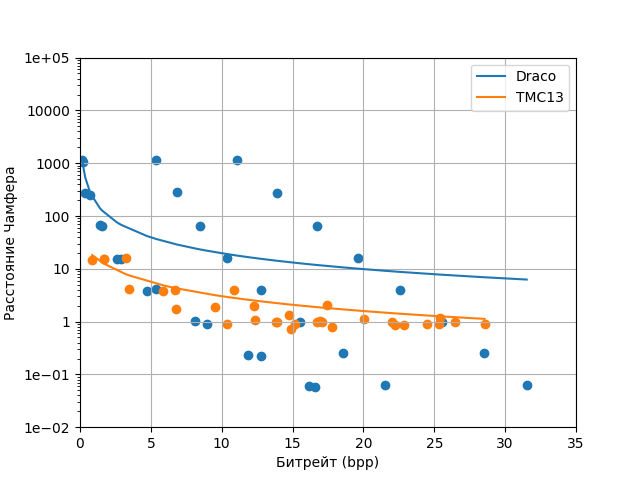
\includegraphics[width=\linewidth]{assets/pcc_arena/approx_cd_p2pt.png}
        \caption{}
    \end{subfigure}
    \begin{subfigure}{0.49\textwidth}
        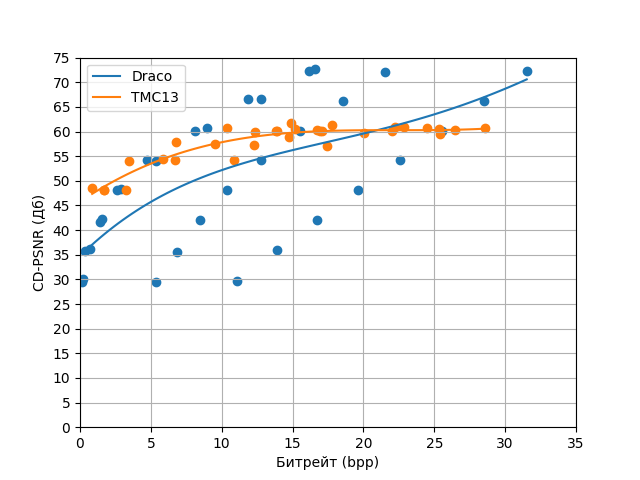
\includegraphics[width=\linewidth]{assets/pcc_arena/approx_cdpsnr_p2pt.png}
        \caption{}
    \end{subfigure}
    \caption{ (a) Зависимость расстояния Чамфера от битрейта. (b) Зависимость
    CD-PSNR от битрейта. }
    \label{img:pcc_arena_cd_bpp}
\end{figure}

На рисунке \ref{img:pcc_arena_cd_bpp} приведен график, изображающий зависимость
расстояния Чамфера от битрейта. По данному графику можно сделать вывод, что
кодек Draco показывает себя хуже относительно TMC13 при низком битрейте. При
высоком битрейте, кодеки показывают схожий результат.

\begin{figure}[H]
    \centering
    \begin{subfigure}{0.49\textwidth}
        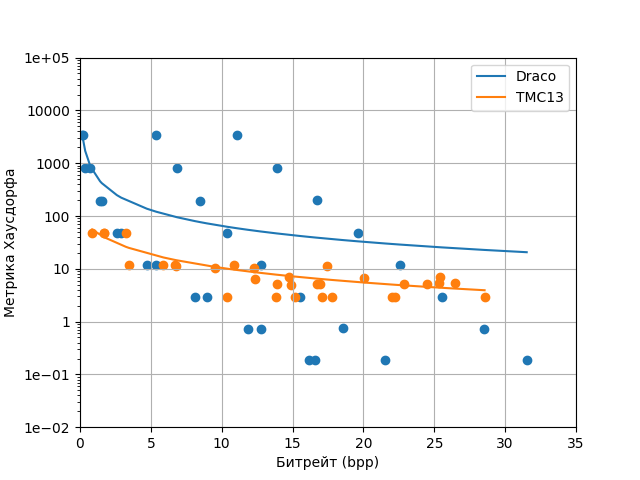
\includegraphics[width=\linewidth]{assets/pcc_arena/approx_h_p2pt.png}
        \caption{}
    \end{subfigure}
    \begin{subfigure}{0.49\textwidth}
        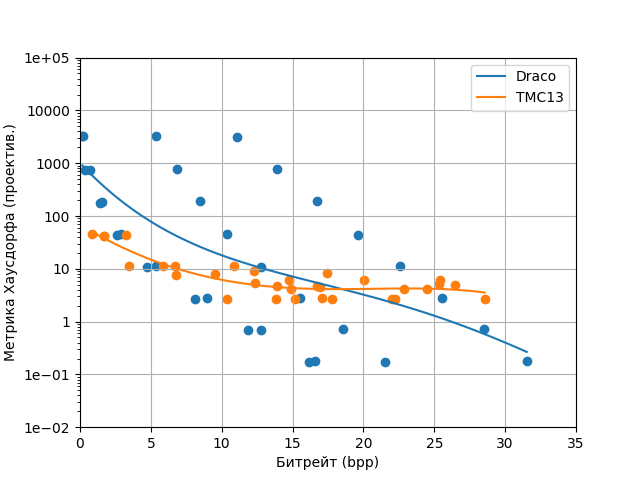
\includegraphics[width=\linewidth]{assets/pcc_arena/approx_h_p2pl.png}
        \caption{}
    \end{subfigure}
    \caption{ (a) Зависимость метрики Хаусдорфа от битрейта. (b) Зависимость
    проецированной метрики Хаусдорфа от битрейта. }
    \label{img:pcc_arena_hd}
\end{figure}

На рисунке \ref{img:pcc_arena_hd} приведен график зависимости метрики Хаусдорфа,
а также значение данной метрики при проецировании вдоль нормалей точек. Данные
графики показывают ошибку метода сжатия в худшем случае, при этом по графику
можно сделать вывод, что соотношение ошибки в худшем случае и в среднем слабо
отличается для приведенных методов сжатия. Кроме того, можно отметить, что при
проецировании ошибки вдоль нормалей, кодек TMC13 показывает незначительно
большее значение метрики Хаусдорфа, при этом значения для кодека Draco остаются
прежними, что может говорить о большем искажении нормалей кодеком TMC13.

\begin{figure}[H]
    \centering
    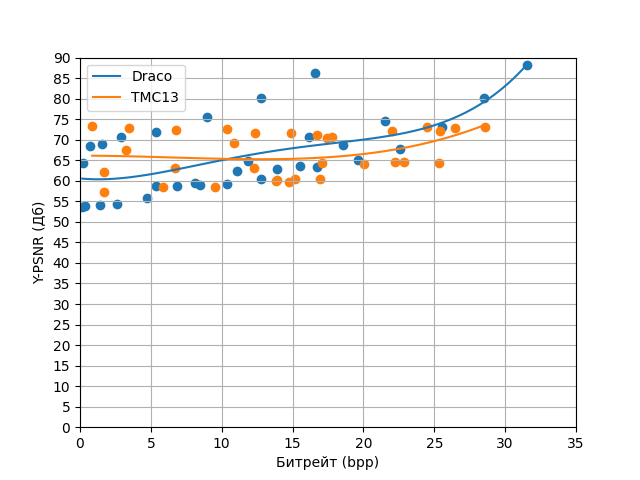
\includegraphics[width=\linewidth]{assets/pcc_arena/approx_y_psnr.png}
    \caption{ Зависимость Y-PSNR от битрейта. }
    \label{img:pcc_arena_y_psnr}
\end{figure}

На графике \ref{img:pcc_arena_y_psnr} приведено отношение пикового сигнала к
шуму для яркостной компоненты цветовой схемы Y'CbCr. По графику можно сделать
вывод, что кодек Draco сильно искажает цвета при малом битрейте, однако, при
повышении битрейта, показывает лучшие значения по сравнению с TMC13. Для TMC13
качество передачи цвета слабо меняется в зависимости от битрейта.

% графикииии





% \chapter{Название главы}
%   \section{Названия секции}
%     \subsection{Название подсекции}
%       \subsection{Название параграфа}
%         \subparagraph{Название подпараграфа}
%           \lipsum[2]\cite{BibExampleRU}
%           \begin{center}
%             \begin{xltabular}{\linewidth}{|l|X|}
%               \caption{Long table caption.\label{long}}                                                                                                    \\
%               \hline
%               Столбик1  & Столбик2    \\
%               \hline
%               слово     & Слово       \\
%               \hline
%             \end{xltabular}
%           \end{center}


% \chapter{Название главы}
%   \section{Названия секции}
%     \subsection{Название подсекции}
%       \subsection{Название Параграфа}
%         \lipsum[2]\cite{BibExampleRU}
%         Как видно на \refImg{img:test} или на \refAppendix{appendix:example}
%         \fig[Длинное название картинки из примера][0.5][img:test]{assets/example.drawio.png}

%         \begin{center}
%           \begin{xltabular}{\linewidth}{|l|X|}
%             \caption{Long table caption.\label{long}}                                                                                                    \\
%             \hline
%             Столбик1  & Столбик2    \\
%             \hline
%             слово     & Слово       \\
%             \hline
%           \end{xltabular}
%         \end{center}

%         \begin{lstlisting}[caption={Название листинга}]
% begin
%   print('Hellow world!')
% end
%         \end{lstlisting}

%         \begin{itemize}
%           \item item1
%           \item item2
%         \end{itemize}

%         \begin{enumerate}
%           \item item1
%           \item item2
%         \end{enumerate}


    \newpage
    \chaperWONum{Заключение}
    В ходе работы были проанализированы существующие подходы к оценке качества
сжатия облаков точек. Был дан подробный обзор предметной области, а также
предложен новый подход к оценке качества сжатия атрибутов облаков точек. Были
сформулированы требования, которым должно удовлетворять проектируемое решение.
Были выбраны технологии и средства разработки для предложенного решения. В
дальнейшем, предложенное решение будет реализовано с использованием выбранных
технологий и средств разработки.



    \newpage
    \chaperWONum{Список источников}
    \printbibliography[heading=none]

    \newpage
    \appendix
    \renewcommand{\thechapter}{\Asbuk{chapter}}
    \addtocontents{toc}{\protect\renewcommand{\protect\chaptername}{Приложение}}
    \chapter{Название приложения}
  \label{appendix:example}
  Текст приложения 1

  \newpage
\chapter{Название приложения}


\end{document}
